\documentclass[12pt,a4paper]{article}
\title{MATH1106 DIS207/208 Quiz 1}
\author{Benjamin Thompson}
\date{February 12, 2020}

\usepackage[margin=1in]{geometry}

\usepackage{amsmath}
\usepackage[usenames,dvipsnames]{xcolor}
\usepackage{tikz}
\usetikzlibrary{arrows.meta,decorations.markings}

\usepackage{fancyhdr}
\pagestyle{fancy}

\fancyhf{}
\lhead{MATH1106 DIS207/208 Quiz 1}
\rhead{February 12, 2020}
\cfoot{\thepage}

\usepackage{enumitem}

\newcommand{\bfa}{\mathbf{a}}
\newcommand{\bfb}{\mathbf{b}}
\newcommand{\bfc}{\mathbf{c}}
\newcommand{\bfd}{\mathbf{d}}


\begin{document}
\subsubsection*{Name:}
Each of the multiple choice question below has one correct choice. Circle the correct choice.
\subsubsection*{Q1}
Two cubes with side length 1cm are glued together along a face to form a rectangular prism of size 2cm $\times$ 1cm $\times$ 1cm. What is the longest possible length between any two points in the rectangular prism? (Recall that the length of a vector $(x,y,z)$ is $\sqrt{x^2 + y^2 + z^2}$).

\begin{enumerate}[label=(\alph*)]
\item $\sqrt{6}$
\item $\sqrt{7}$
\item $\sqrt{8}$
\item $3$
\end{enumerate}

\subsubsection*{Q2}
Several vectors are plotted below.
\[
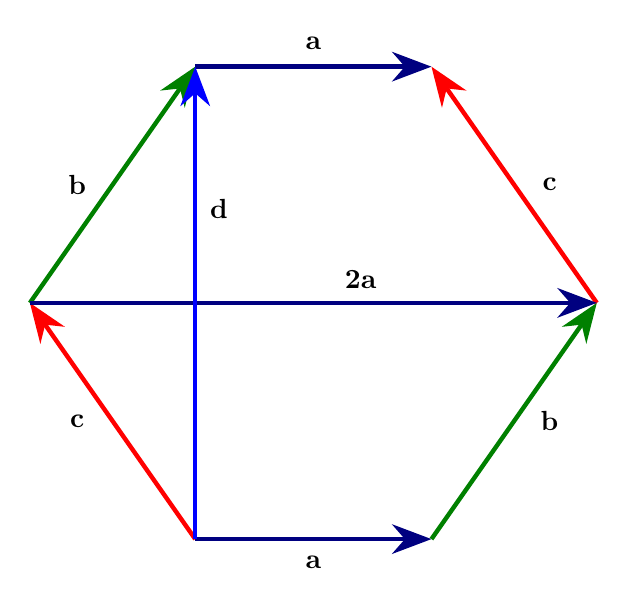
\begin{tikzpicture}[auto,ultra thick,scale=3]

\node (bm) at (0.5,-0.1) {$\mathbf{a}$};
\node (mm) at (0.7,1.1) {$\mathbf{2a}$};
\node (tm) at (0.5,2.1) {$\mathbf{a}$};

\node (br) at (1.5,0.5) {$\mathbf{b}$};
\node (tl) at (-0.5,1.5) {$\mathbf{b}$};

\node (bl) at (-0.5,0.5) {$\mathbf{c}$};
\node (tr) at (1.5,1.5) {$\mathbf{c}$};

\node (vt) at (0.1,1.4) {$\mathbf{d}$};

\draw[NavyBlue,-{Stealth[length=5mm]}] (0,0) -- (1,0);
\draw[NavyBlue,-{Stealth[length=5mm]}] (0,2) -- (1,2);

\draw[Green,-{Stealth[length=5mm]}] (1,0) -- (1.7,1);
\draw[Green,-{Stealth[length=5mm]}] (-0.7,1) -- (0,2);

\draw[Red,-{Stealth[length=5mm]}] (0,0) -- (-0.7,1);
\draw[Red,-{Stealth[length=5mm]}] (1.7,1) -- (1,2);

\draw[NavyBlue,-{Stealth[length=5mm]}] (-0.7,1) -- (1.7,1);
\draw[Blue,-{Stealth[length=5mm]}] (0,0) -- (0,2);
\end{tikzpicture}
\]
Which of the following correctly describes $\mathbf{c}$ and $\mathbf{d}$ in terms of $\bfa$ and $\mathbf{b}$?

\begin{enumerate}[label=(\alph*)]
\item $\bfc = 2\bfa - \bfb$, $\bfd = -\bfa + 2\bfb$
\item $\bfc = \bfb - \bfa$, $\bfd = -\bfa + 2\bfb$
\item $\bfc = 2\bfa - \bfb$, $\bfd = 2\bfb - 2\bfa$
\item $\bfc = \bfb - \bfa$, $\bfd = 2\bfa + \bfb$
\end{enumerate}

\newpage

\subsubsection*{Q3}
Assume a feral camel population in an Australian National Park is modeled by the logistic equation
\[
	X' = 1000X - 0.2X^2.
\]
Which of the following about the camel population is predicted by the model?

\begin{table}[ht!]
	\centering
	\begin{tabular}{|c|c|c|}
	\hline
	& $X = 500$ & $X = 6000$ \\
	\hline
	(a) & the population is increasing & the population is increasing \\
	\hline
	(b) & the population is increasing & the population is decreasing \\
	\hline
	(c) & the population is stable & the population is decreasing \\
	\hline
	(d) & the population is decreasing & the population is decreasing \\
	\hline
	\end{tabular}
\end{table}

\subsubsection*{Q4}
Which of the following is a differential equation for the following verbal statement: the yearly rate of change of a population is the sum of births, deaths, immigration, and emigration, with per capita birth rate 17.5, per capita death rate 7.1, immigration rate of 20000 individuals per year, and per capita emigration rate 0.4.

\begin{enumerate}[label=(\alph*)]
\item $P' = 20010$
\item $P' = 20010P$
\item $P' = 10P + 20000$
\item $P' = 10.8P - 20000$
\end{enumerate}

\subsubsection*{Q5}
Which of the following pairs of equations are an example of Lotka-Volterra predator-prey equations, assuming $X$ represents the number of prey and $Y$ represents the number of predators?

\begin{table}[ht!]
	\centering
	\begin{tabular}{|c|c|c|}
	\hline
	(a) & $X' = 2.1X + 0.5XY $& $Y' = -0.1Y + 3XY$\\
	\hline
	(b) & $X' = 2.1X - 0.5XY$& $Y' = -0.1Y + 3XY$\\
	\hline
	(c) & $X' = -0.1X + 3XY$& $Y' = 2.1Y - 0.5XY$\\
	\hline
	(d) & $X' = -0.1X + 3XY$& $Y' = 2.1Y + 0.5XY$\\
	\hline
	\end{tabular}
\end{table}
\end{document}
